\chapter{Cómo se construyó el bosque}

\begin{enpocas}
Cómo se generaron por programa el terreno con montañas, su textura, los 1700 árboles, las rocas, los animales y el incendio con humo, y cómo los arma el \emph{launch} al arrancar.
\end{enpocas}

\section{Mundos disponibles}

\begin{description}
  \item[\cod{incendio}] terreno plano, tres árboles simples y el foco en $(8,5)$. Sirve para
        probar el control sin distracciones.
  \item[\cod{bosque}] como el del video de ArduPilot \cod{iris_forest}: 50 robles y 35 pinos de
        OpenRobotics (Gazebo Fuel, licencia CC0, copiados en \cod{models/roble} y
        \cod{models/pino} para funcionar sin internet) y el foco en $(8,5)$. Deja libres el
        despegue, el corredor al foco y el anillo de la órbita, así que la misión \cod{orbita}
        funciona a 3~m entre los árboles. Se genera con
        \cod{python3 scripts/generar_bosque.py worlds/bosque.sdf} (semilla fija).
  \item[\cod{bosque_grande}] el valle boscoso con montañas que se describe a continuación.
\end{description}

\section{El mundo \texorpdfstring{\texttt{bosque\_grande}}{bosque\_grande}}

\begin{figure}[H]
\centering
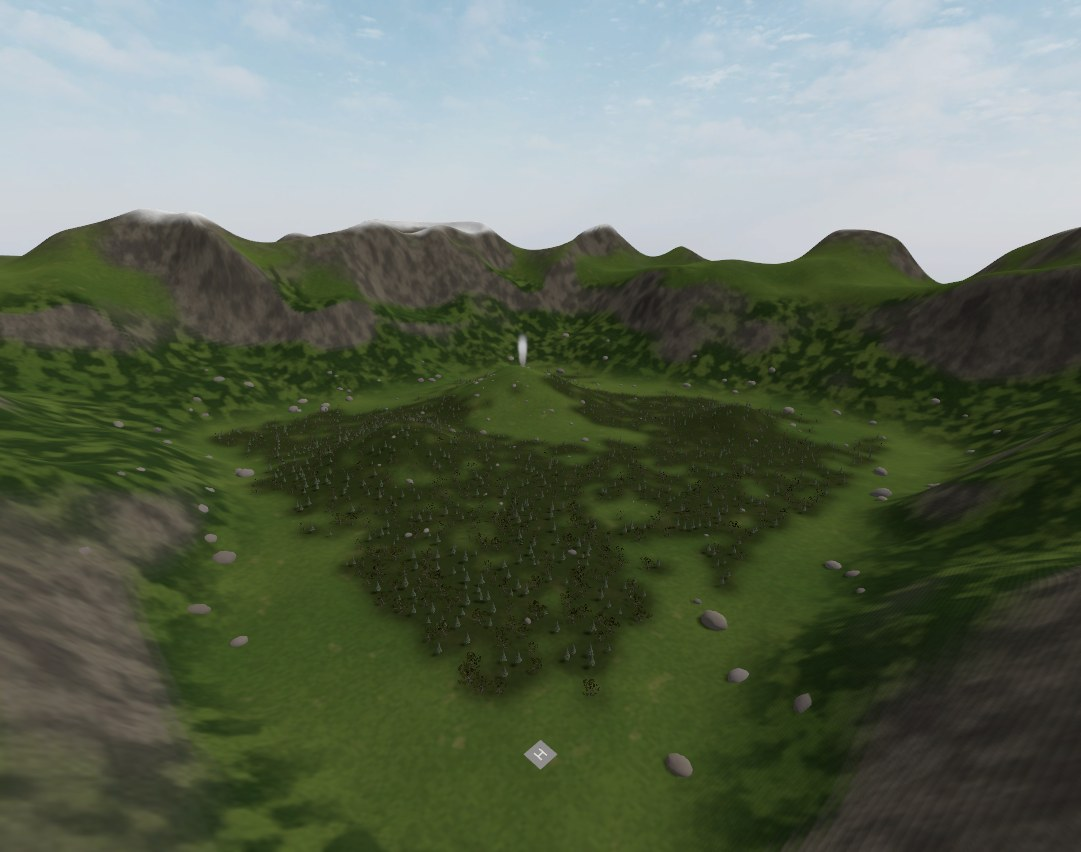
\includegraphics[width=\textwidth]{gz_valle_aereo.jpg}
\caption{Vista aérea del valle desde el suroeste. Abajo al centro, la base de despegue; al
fondo, el penacho de humo del incendio.}
\end{figure}

Se pidió ``un mundo más grande, con más árboles, montañas, piedras grandes, cielo y animales,
en el que el dron monitoree todo el bosque para encontrar el incendio''. El resultado:

\begin{itemize}
  \item Terreno de $1.2\times1.2$~km con malla de 4~m ($301\times301$ vértices). El valle mide
        $420\times420$~m, con lomas suaves y tres cerros de 18 a 42~m; alrededor, una cordillera
        de hasta $\approx$215~m con laderas de roca y nieve en las cumbres.
  \item Textura propia de $4096\times4096$ píxeles.
  \item 1700 árboles (956 pinos y 744 robles) de tamaños y orientaciones variables, con claros de
        pastizal; miden de 4.6 a 8.2~m.
  \item 140 rocas y peñascos.
  \item 21 animales (venados, lobos y zorros) que pastan y caminan.
  \item Cielo con nubes (\cod{<sky>} de Gazebo).
  \item Base de despegue de $8\times8$~m con una ``H'' en $(-232,-232)$, fuera del bosque.
  \item Foco de incendio por omisión en una ladera al noreste, $(105,135)$, con un claro
        quemado de 9~m y un penacho de humo de $\approx$30~m que se ve sobre las copas.
\end{itemize}

\subsection{Generación del terreno}

Todo lo genera una sola vez, con semilla fija (21), el script:
\begin{lstlisting}[style=bash]
~/.venvs/cad/bin/python scripts/generar_bosque_grande.py
\end{lstlisting}

\begin{enumerate}
  \item \textbf{Relieve} (\cod{alturas}). Suma de: ruido fractal suave de amplitud 7~m (lomas),
        tres gaussianas deformadas por ruido (los cerros), y la cordillera, que crece con la
        distancia al borde del valle. El borde es un cuadrado redondeado de 250~m de semilado
        ($|x|^6+|y|^6$) deformado por ruido para que no se vea artificial; las crestas salen de
        $1-|\text{ruido}|$. Se suaviza con un filtro gaussiano ($\sigma = 1.2$ celdas) y se aplana la
        base de despegue.
  \item \textbf{Textura} (\cod{colores_textura}). Por cada píxel: dos verdes de pasto mezclados con
        ruido, manchas secas, sotobosque oscuro bajo las copas (según la densidad de árboles),
        monte denso en las faldas, roca donde la pendiente pasa de $\approx$0.8 o la altura de
        140~m, y nieve por encima de 185~m.
  \item \textbf{Árboles} (\cod{distribuir_arboles}). Puntos al azar en la zona, descartando:
        cerca de las montañas (el bosque se ralea), en los claros (donde el ruido es bajo), a menos
        de 30~m de la base, con pendiente mayor a 0.75 o por encima de 95~m, y donde se
        encimarían con otro árbol. Hay más pinos cuanto más alto.
  \item \textbf{Rocas.} Icoesferas deformadas, exportadas \emph{con normales} (ver el recuadro).
  \item \textbf{Fauna.} Grupos de animales en los claros.
\end{enumerate}

Deja en \cod{models/terreno_bosque_grande/}: la malla (\cod{terreno.obj}, también como colisión),
la textura (\cod{suelo.jpg}), el DEM (\cod{altura.npz}), las rocas, la lista de objetos
(\cod{objetos.json}) y el \cod{model.sdf}.

\begin{figure}[H]
\centering
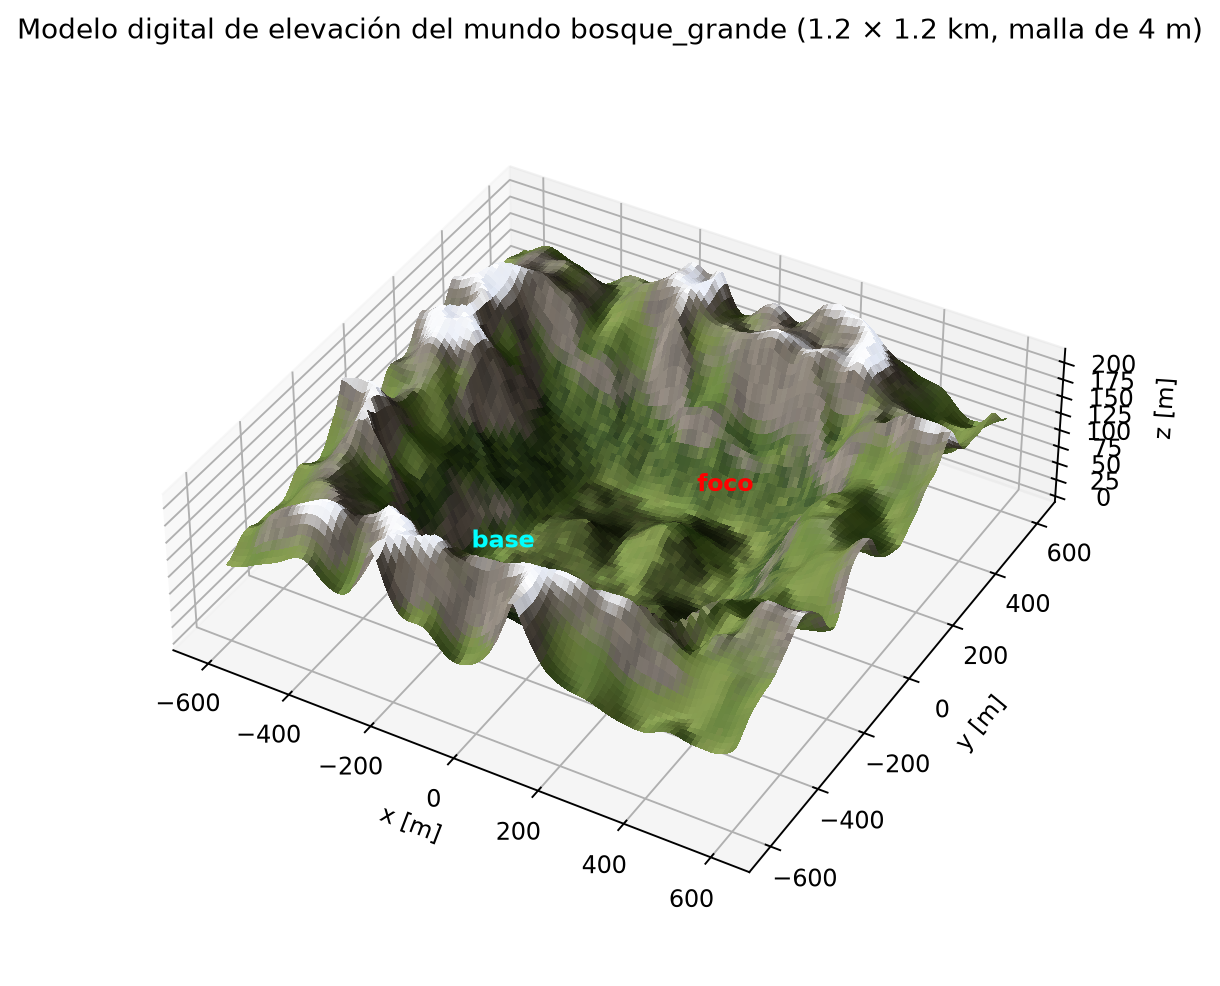
\includegraphics[width=0.9\textwidth]{dem_3d.png}
\caption{Modelo digital de elevación con la textura generada.}
\label{fig:dem}
\end{figure}

\begin{leccion}
La primera versión hacía que Gazebo se cayera con \emph{segfault} en
\cod{OdeMesh::fillArrays} en cuanto el dron tocaba algo. La causa: las mallas OBJ de colisión de las
rocas no traían normales. Se resolvió exportándolas con normales.
\end{leccion}

\subsection{El DEM y la clase \texttt{Terreno}}

\cod{altura.npz} guarda $x_0$, $y_0$, el paso y la matriz $h[i_y, i_x]$. \cod{cuadrirotor_sim/terreno.py}
interpola por triángulos (con la diagonal $(i_x,i_y)$--$(i_x{+}1,i_y{+}1)$, igual que la malla de
Gazebo) y ofrece:
\begin{itemize}
  \item \cod{altura(x, y)}: altura del suelo (vectorizada);
  \item \cod{maximo_en_tramo(a, b)}: punto más alto entre dos puntos (para seguir el relieve);
  \item \cod{cortar_rayo(o, d, alcance, desfase)}: dónde un rayo de la cámara toca el suelo.
\end{itemize}
Lo usan el planificador, la fauna (para caminar sobre el suelo, inclinados según la pendiente), el
\emph{launch} (para poner el dron y el foco sobre el terreno) y la captura de datos (para saber
qué tapa el relieve). Sin DEM, el suelo es el plano $z = 0$.

\subsection{Árboles en un solo modelo}

Para que 1700 árboles corran a tiempo real, todos van en un único modelo estático \cod{bosque}:
cada árbol es un \emph{visual} escalado (copa y corteza de la malla de OpenRobotics) y su
colisión es solo un cilindro en el tronco. Las rocas van igual en un modelo \cod{rocas}.

\subsection{Fauna}

Los modelos son CC0 de OpenGameArt: venado (crownjoshua), zorro y lobo (Quaternius).
\cod{scripts/preparar_fauna.py} los descarga, los gira a ``$z$ arriba y la cabeza hacia $+x$'',
los escala (venado 1.55~m, zorro 0.55~m, lobo 0.95~m), les pone colores por parte y los exporta a
\cod{models/fauna_*} (dinámicos, sin gravedad ni colisión). Se descartó un águila porque traía las
alas caídas.

El nodo \cod{fauna} (sin ROS, solo gz-transport) mueve a todos los animales con el servicio
\cod{/world/bosque_grande/set_pose_vector} a 10~Hz de tiempo simulado: alternan pausas (pastar,
olfatear) con caminatas a un punto al azar de su territorio; los lobos y zorros a veces trotan.

\begin{figure}[H]
\centering
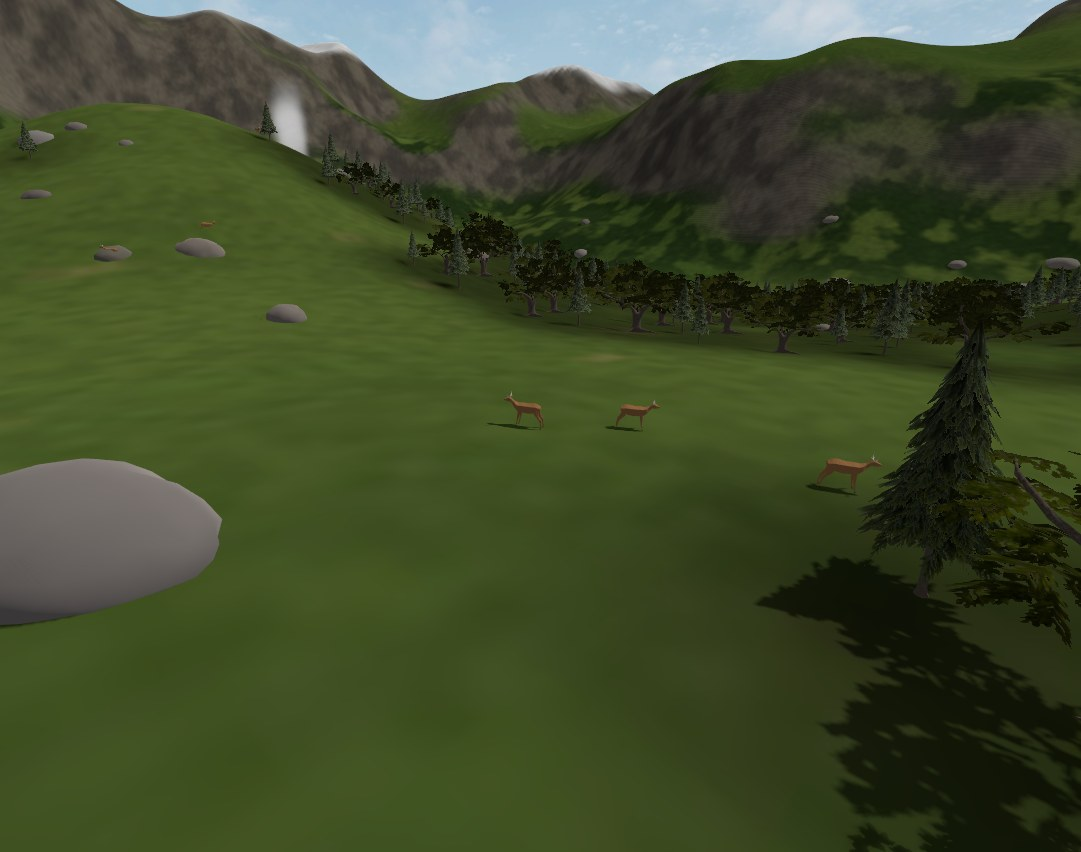
\includegraphics[width=0.49\textwidth]{gz_fauna.jpg}\hfill
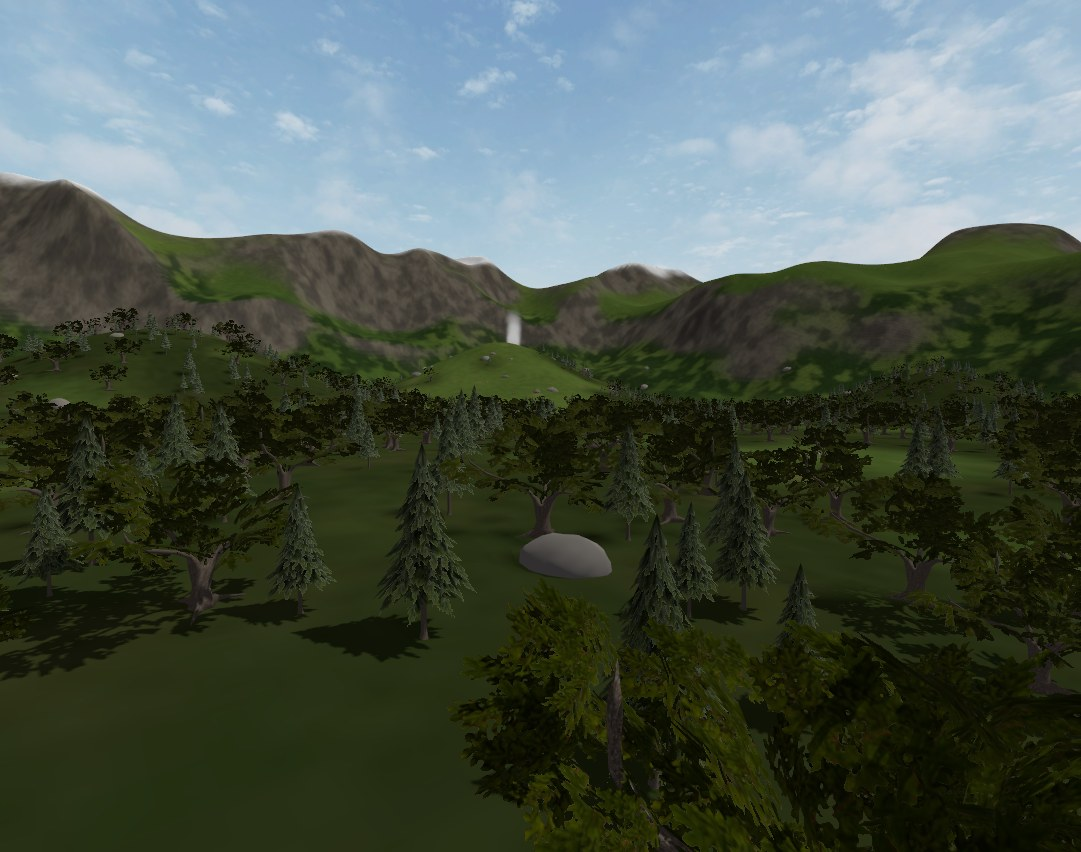
\includegraphics[width=0.49\textwidth]{gz_bosque_bajo.jpg}
\caption{Venados pastando en un claro (izquierda) y el bosque visto a baja altura (derecha).}
\end{figure}

\section{El incendio}

\cod{python3 scripts/generar_fuego.py} genera las texturas de las partículas y dos modelos:
\begin{itemize}
  \item \cod{foco_incendio}: siete emisores de llama (blanco amarillento $\rightarrow$ naranja
        $\rightarrow$ rojo $\rightarrow$ transparente), una columna de humo que crece y se aclara al
        subir, brasas, troncos carbonizados, suelo quemado y una luz naranja;
  \item \cod{columna_humo}: el penacho alto ($\approx$30~m, vida de 26~s) para el mundo grande.
\end{itemize}
Usan el sistema \cod{gz-sim-particle-emitter-system}; son solo visuales (no colisionan).

\begin{aviso}
Gazebo solo encuentra la imagen de rango de colores de las partículas
(\cod{<color_range_image>}) con una ruta absoluta. Por eso el \emph{launch} copia los dos modelos a
\cod{/tmp/cuadrirotor_sim_<uid>/modelos} con las rutas resueltas al arrancar.
\end{aviso}

\begin{figure}[H]
\centering
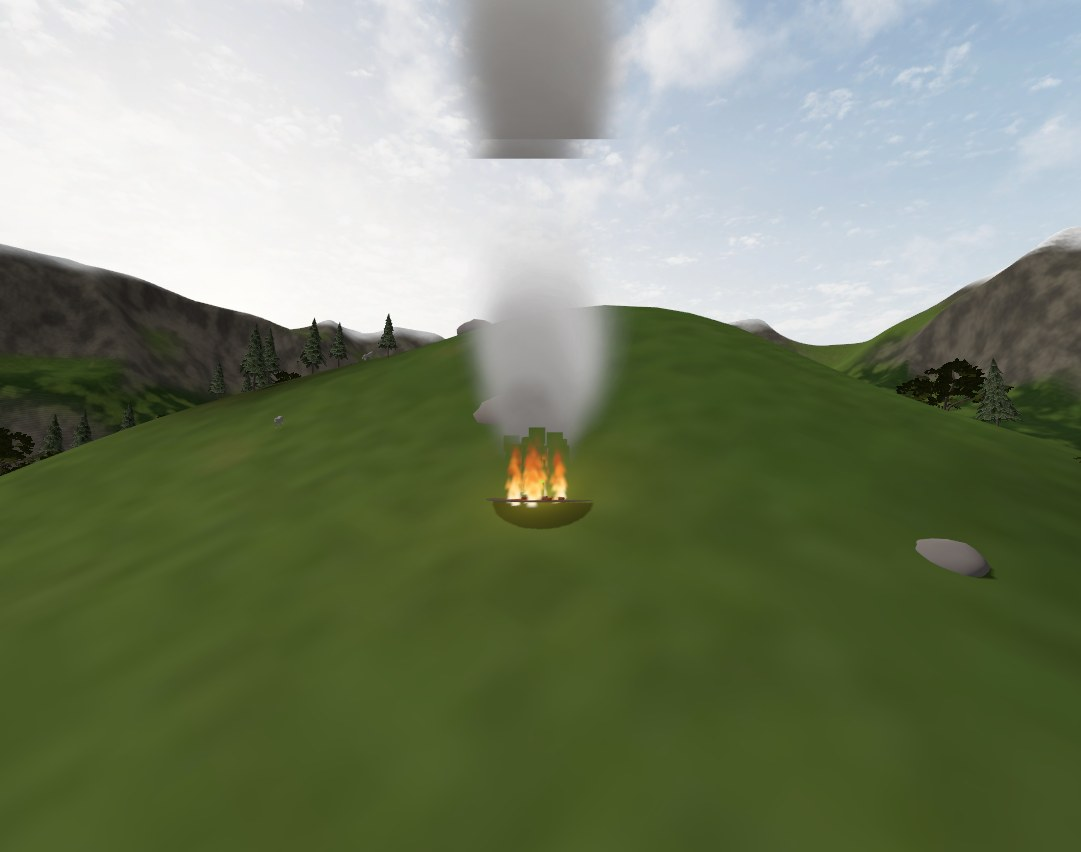
\includegraphics[width=0.62\textwidth]{gz_foco_cerca.jpg}
\caption{El foco de incendio en la ladera: llamas, claro quemado y columna de humo.}
\end{figure}

\section{Cómo arma el mundo el \emph{launch}}

Con \cod{mundo:=bosque_grande} el \emph{launch} (\cod{simulacion.launch.py}) escribe el SDF al
arrancar en \cod{/tmp/cuadrirotor_sim_<uid>/bosque_grande.sdf}, con el foco en
(\cod{foco_x}, \cod{foco_y}) sobre el terreno y el claro quemado alrededor
(\cod{cuadrirotor_sim/bosque_grande.py}). También:
\begin{itemize}
  \item pone el vehículo en la base, a la altura del DEM más 5~cm;
  \item lanza el nodo \cod{fauna};
  \item con GUI, arranca la cámara cerca de la base y a los 12~s llama a \cod{/gui/follow} y
        \cod{/gui/follow/offset} para que siga al dron;
  \item pasa al planificador \cod{config/mundo_bosque_grande.yaml} y la ruta del DEM.
\end{itemize}

El mundo está georreferenciado para que el GPS de Gazebo y el de ArduPilot coincidan con el aviso
del incendio (sección~\ref{sec:gps}):
\begin{lstlisting}[style=xml]
<spherical_coordinates>
  <surface_model>EARTH_WGS84</surface_model>
  <world_frame_orientation>ENU</world_frame_orientation>
  <latitude_deg>19.293</latitude_deg>
  <longitude_deg>-99.311</longitude_deg>
  <elevation>3000.0</elevation>
  <heading_deg>0</heading_deg>
</spherical_coordinates>
\end{lstlisting}

\begin{lstlisting}[style=bash]
# Foco en otro lugar del valle:
ros2 launch cuadrirotor_sim simulacion.launch.py vehiculo:=tarot650 mundo:=bosque_grande \
    controlador:=sta mision:=busqueda foco_x:=-150 foco_y:=60
\end{lstlisting}
